\documentclass[aspectratio=169,11pt]{beamer}

\usepackage[utf8]{inputenc}
\usepackage[T1]{fontenc}
\usepackage[spanish,es-tabla,es-nodecimaldot]{babel}
\usepackage{lmodern}
\usepackage{booktabs}
\usepackage{graphicx}

\graphicspath{{figures/}}
% Archivo generado automáticamente por notebooks/01_eda.ipynb -- no editar a mano
\newcommand{\nClips}{1440}
\newcommand{\nActores}{24}
\newcommand{\nEmociones}{8}
\newcommand{\nClipsNeutral}{96}
\newcommand{\nClipsOtras}{192}
\newcommand{\nEstereo}{5}
\newcommand{\tamanoMB}{590.3}
\newcommand{\durMedia}{3.7}
\newcommand{\durMin}{2.9}
\newcommand{\durMax}{5.3}
\newcommand{\durVozMedia}{1.9}
\newcommand{\silInicio}{0.937}
\newcommand{\silFinal}{0.893}
\newcommand{\fracSilencio}{49.8}
\newcommand{\foHombre}{149.3}
\newcommand{\foMujer}{256.9}
\newcommand{\rmsNormal}{0.009}
\newcommand{\rmsFuerte}{0.023}
\newcommand{\rmsRatio}{2.6}
\newcommand{\emoMaxRMS}{enojo}
\newcommand{\emoMinRMS}{calma}
\newcommand{\rmsMaxVal}{0.037}
\newcommand{\rmsMinVal}{0.004}
\newcommand{\emoMaxFo}{miedo}
\newcommand{\emoMinFo}{calma}
\newcommand{\foMaxVal}{270.7}
\newcommand{\foMinVal}{160.5}
\newcommand{\emoMaxDur}{asco}
\newcommand{\emoMinDur}{sorpresa}
\newcommand{\pcUno}{29.2}
\newcommand{\pcDos}{13.5}
\newcommand{\nPCNoventa}{15}
\newcommand{\nDescriptores}{30}
\newcommand{\frameLen}{2048}
\newcommand{\hopLen}{512}
\newcommand{\ventanaMs}{92.9}
\newcommand{\saltoMs}{23.2}
\newcommand{\nMujer}{720}
\newcommand{\nHombre}{720}
\newcommand{\atipTotalMujer}{120}
\newcommand{\atipTotalHombre}{111}
\newcommand{\atipMaxDesc}{RMS}
\newcommand{\kwTop}{Energía RMS media}
\newcommand{\kwTopEps}{0.446}
\newcommand{\kwLow}{Tasa de cruces por cero}
\newcommand{\kwLowEps}{0.117}
\newcommand{\tablaKruskal}{%
Energía RMS media & 645.5 & $<10^{-10}$ & 0.446 \\
Duración de voz (s) & 296.0 & $<10^{-10}$ & 0.202 \\
F0 media (Hz) & 290.9 & $<10^{-10}$ & 0.198 \\
Centroide espectral (Hz) & 248.3 & $<10^{-10}$ & 0.169 \\
Rango de F0 p5–p95 (Hz) & 239.7 & $<10^{-10}$ & 0.162 \\
Tasa de cruces por cero & 174.4 & $<10^{-10}$ & 0.117 \\
}
\newcommand{\tablaMedianas}{%
neutral & 1.63 & 0.006 & 0.104 & 2056 & 177 \\
calma & 1.95 & 0.004 & 0.114 & 2220 & 161 \\
alegría & 1.72 & 0.019 & 0.113 & 2250 & 239 \\
tristeza & 1.82 & 0.007 & 0.116 & 2192 & 203 \\
enojo & 1.89 & 0.037 & 0.140 & 2544 & 262 \\
miedo & 1.68 & 0.024 & 0.125 & 2527 & 271 \\
asco & 2.04 & 0.010 & 0.138 & 2476 & 199 \\
sorpresa & 1.60 & 0.016 & 0.122 & 2407 & 265 \\
}
\newcommand{\tablaAtipicos}{%
ZCR & 11 & 1.5\,\% & 17 & 2.4\,\% \\
RMS & 75 & 10.4\,\% & 75 & 10.4\,\% \\
MFCC1 & 0 & 0.0\,\% & 1 & 0.1\,\% \\
MFCC2 & 13 & 1.8\,\% & 9 & 1.2\,\% \\
MFCC3 & 12 & 1.7\,\% & 3 & 0.4\,\% \\
MFCC4 & 9 & 1.2\,\% & 6 & 0.8\,\% \\
}
\newcommand{\tablaFrameHop}{%
512 & 128 & 23.2 & 5.8 & 431 \\
1024 & 256 & 46.4 & 11.6 & 216 \\
2048 & 512 & 92.9 & 23.2 & 108 \\
4096 & 1024 & 185.8 & 46.4 & 54 \\
}


% ---------- Estilo ----------
\usetheme{default}
\definecolor{acento}{HTML}{1C5CAB}
\definecolor{tinta}{HTML}{0B0B0B}
\definecolor{tinta2}{HTML}{52514E}
\definecolor{fondo2}{HTML}{F0EFEC}
\setbeamercolor{frametitle}{fg=acento}
\setbeamercolor{title}{fg=acento}
\setbeamercolor{structure}{fg=acento}
\setbeamercolor{normal text}{fg=tinta}
\setbeamercolor{block title}{bg=acento,fg=white}
\setbeamercolor{block body}{bg=fondo2}
\setbeamerfont{frametitle}{series=\bfseries,size=\Large}
\setbeamerfont{title}{series=\bfseries,size=\LARGE}
\setbeamertemplate{navigation symbols}{}
\setbeamertemplate{itemize items}[circle]
\setbeamertemplate{enumerate items}[default]
\setbeamertemplate{footline}{%
  \hspace{1em}{\color{tinta2}\tiny RAVDESS · Análisis exploratorio}\hfill
  {\color{tinta2}\tiny\insertframenumber/\inserttotalframenumber}\hspace{1em}\vspace{0.6em}}
\newcommand{\nota}[1]{{\small\color{tinta2}#1}}

\title{Reconocimiento de emociones en la voz}
\subtitle{Análisis exploratorio del corpus RAVDESS (habla)}
\author{Saúl Ubaldo Rojas Vázquez \and Karols Cisneros \and Mónica}
\date{\today}

\begin{document}

\begin{frame}[plain]
  \titlepage
\end{frame}

% ===================== OBJETIVOS =====================
\section{Objetivos}
\begin{frame}{Objetivos}
  \begin{block}{Objetivo general}
    Caracterizar el corpus RAVDESS (habla) para fundamentar un modelo de clasificación de emociones a
    partir de la voz.
  \end{block}
  \vspace{0.6em}
  \textbf{Objetivos específicos}
  \begin{enumerate}
    \item Publicar el corpus en Supabase para consumirlo sin copias locales.
    \item Verificar la integridad y la calidad de los datos.
    \item Describir su composición por emoción, intensidad, género y actor.
    \item Identificar los descriptores acústicos que distinguen emociones.
    \item Detectar fuentes de variación ajenas a la emoción.
  \end{enumerate}
\end{frame}

% ===================== DATASET =====================
\section{Dataset}
\begin{frame}{Dataset: RAVDESS}
  \begin{columns}[T]
    \begin{column}{0.48\textwidth}
      \begin{itemize}
        \item \textbf{\nActores{} actores} profesionales (12 H / 12 M)
        \item \textbf{\nEmociones{} emociones}: neutral, calma, alegría, tristeza, enojo, miedo, asco,
              sorpresa
        \item 2 intensidades, 2 frases, 2 repeticiones
        \item Subconjunto de \textbf{audio de habla}: \nClips{} WAV, 48\,kHz, \tamanoMB\,MB
      \end{itemize}
      \vspace{0.4em}
      \nota{Frases: ``Kids are talking by the door'' / ``Dogs are sitting by the door''.}
    \end{column}
    \begin{column}{0.5\textwidth}
      \textbf{Metadatos en el nombre del archivo}\\[0.3em]
      \centering\texttt{03-01-05-02-01-01-07.wav}\\[0.4em]
      \footnotesize
      \begin{tabular}{@{}ll@{}}
        \toprule
        03 & solo audio \\
        01 & habla \\
        05 & enojo \\
        02 & intensidad fuerte \\
        01 & frase ``Kids'' \\
        01 & repetición 1 \\
        07 & actor 7 (impar = hombre) \\
        \bottomrule
      \end{tabular}
    \end{column}
  \end{columns}
\end{frame}

\begin{frame}{Datos en Supabase}
  \begin{columns}[T]
    \begin{column}{0.5\textwidth}
      \textbf{Storage} — bucket \texttt{ravdess-audio}
      \begin{itemize}
        \item \nClips{} WAV en \texttt{Actor\_XX/<archivo>.wav}
        \item Lectura pública por URL
      \end{itemize}
      \vspace{0.5em}
      \textbf{PostgreSQL} — tabla \texttt{ravdess\_clips}
      \begin{itemize}
        \item Una fila por clip: actor, género, emoción, intensidad, frase, duración, etc.
        \item RLS activo: solo lectura para roles públicos
      \end{itemize}
    \end{column}
    \begin{column}{0.46\textwidth}
      \begin{block}{Verificación de la carga}
        \nClips{} objetos $=$ \nClips{} filas\\
        0 archivos faltantes\\
        Tamaño idéntico a la fuente
      \end{block}
      \vspace{0.4em}
      \nota{Los notebooks leen la tabla vía API REST y descargan el audio bajo demanda a una caché
      temporal.}
    \end{column}
  \end{columns}
\end{frame}

% ===================== EDA =====================
\section{EDA}
\begin{frame}{Calidad y composición}
  \begin{columns}[c]
    \begin{column}{0.64\textwidth}
      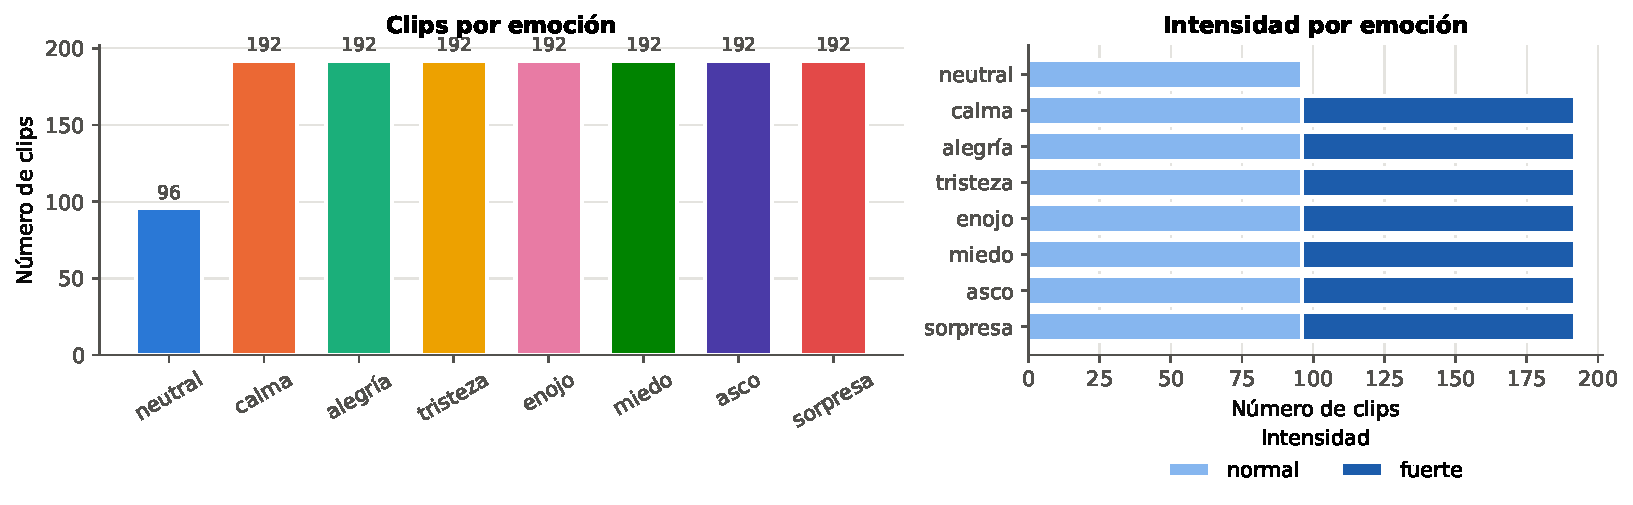
\includegraphics[width=\linewidth]{distribucion_emociones}
    \end{column}
    \begin{column}{0.34\textwidth}
      \small
      \begin{itemize}
        \item Sin nulos ni duplicados
        \item \nEstereo{} clips estéreo $\rightarrow$ mono
        \item 60 clips por actor; 720 por género
        \item \textbf{Neutral: \nClipsNeutral{} vs.\ \nClipsOtras} (sin intensidad fuerte)
      \end{itemize}
    \end{column}
  \end{columns}
\end{frame}

\begin{frame}{Frame length y hop length}
  \begin{columns}[c]
    \begin{column}{0.6\textwidth}
      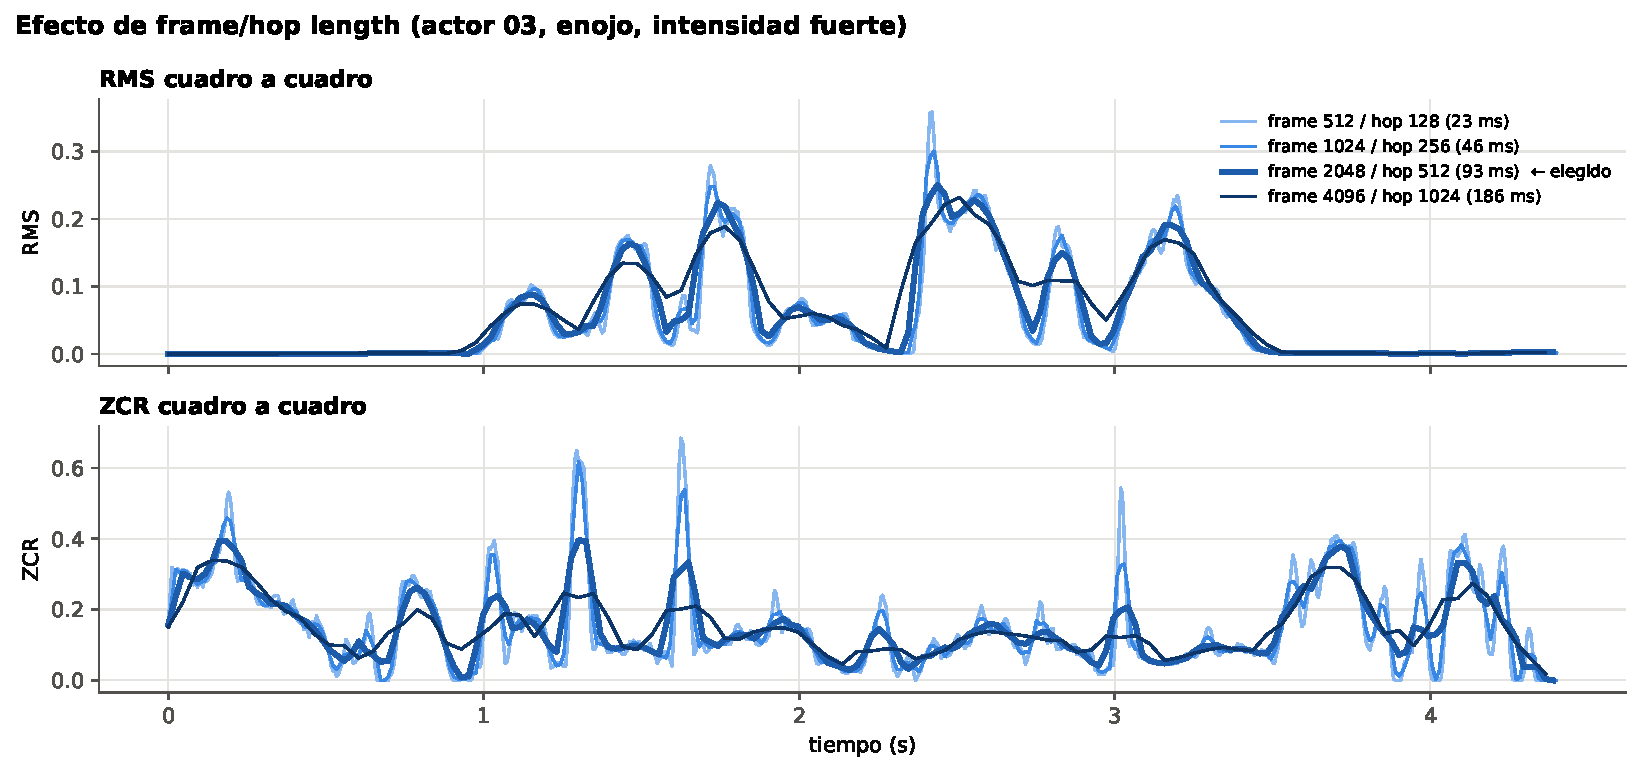
\includegraphics[width=\linewidth]{frame_hop_length}
    \end{column}
    \begin{column}{0.38\textwidth}
      \footnotesize
      MFCC, ZCR y RMS se calculan \textbf{cuadro a cuadro}.\\[0.4em]
      {\scriptsize\setlength{\tabcolsep}{4pt}
      \begin{tabular}{@{}rrrrr@{}}
        \toprule
        Frame & Hop & ms & ms & Cuadros \\
        \midrule
        \tablaFrameHop
        \bottomrule
      \end{tabular}}\\[0.5em]
      \textbf{Elegido: \frameLen/\hopLen} (\ventanaMs/\saltoMs\,ms). 512 da curvas ruidosas y 4096 borra
      los picos silábicos.
    \end{column}
  \end{columns}
\end{frame}

\begin{frame}{Duración y silencios}
  \centering
  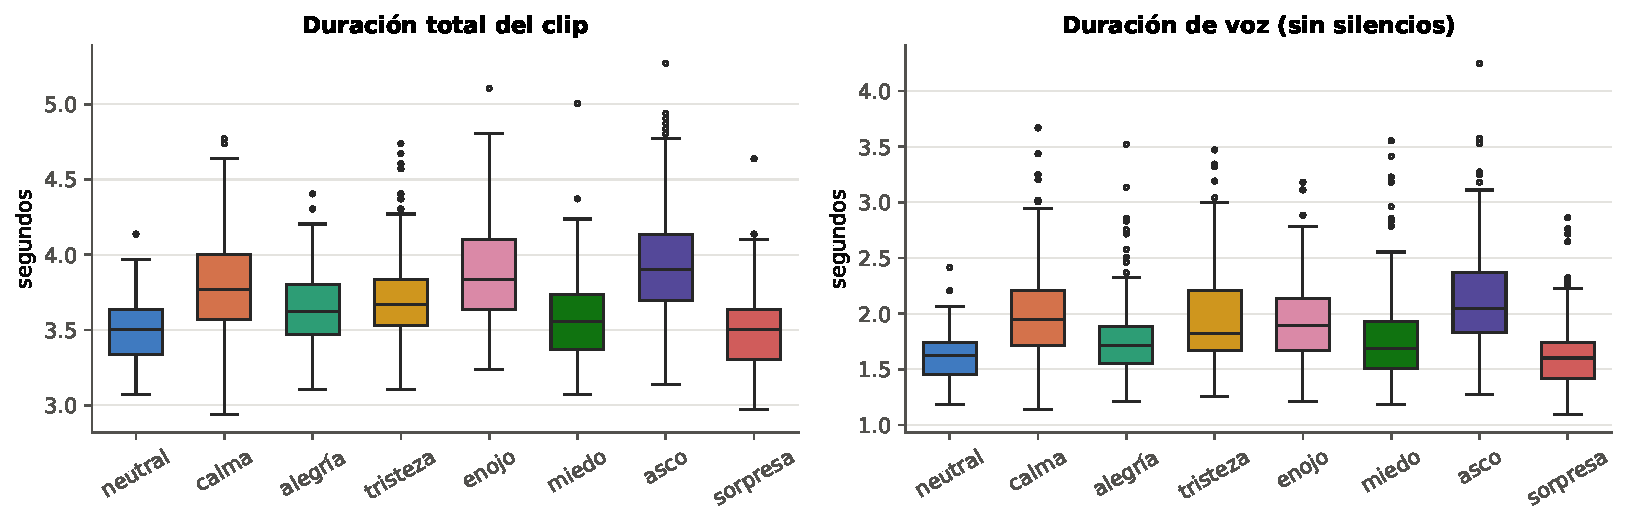
\includegraphics[width=0.92\linewidth]{duraciones}\\[0.3em]
  \small Clips de \durMin--\durMax\,s; \textbf{\fracSilencio\,\% es silencio}
  (\silInicio\,s al inicio, \silFinal\,s al final). Voz efectiva: \durVozMedia\,s.
\end{frame}

\begin{frame}{Waveplot por emoción y género}
  \begin{columns}[c]
    \begin{column}{0.55\textwidth}
      \centering
      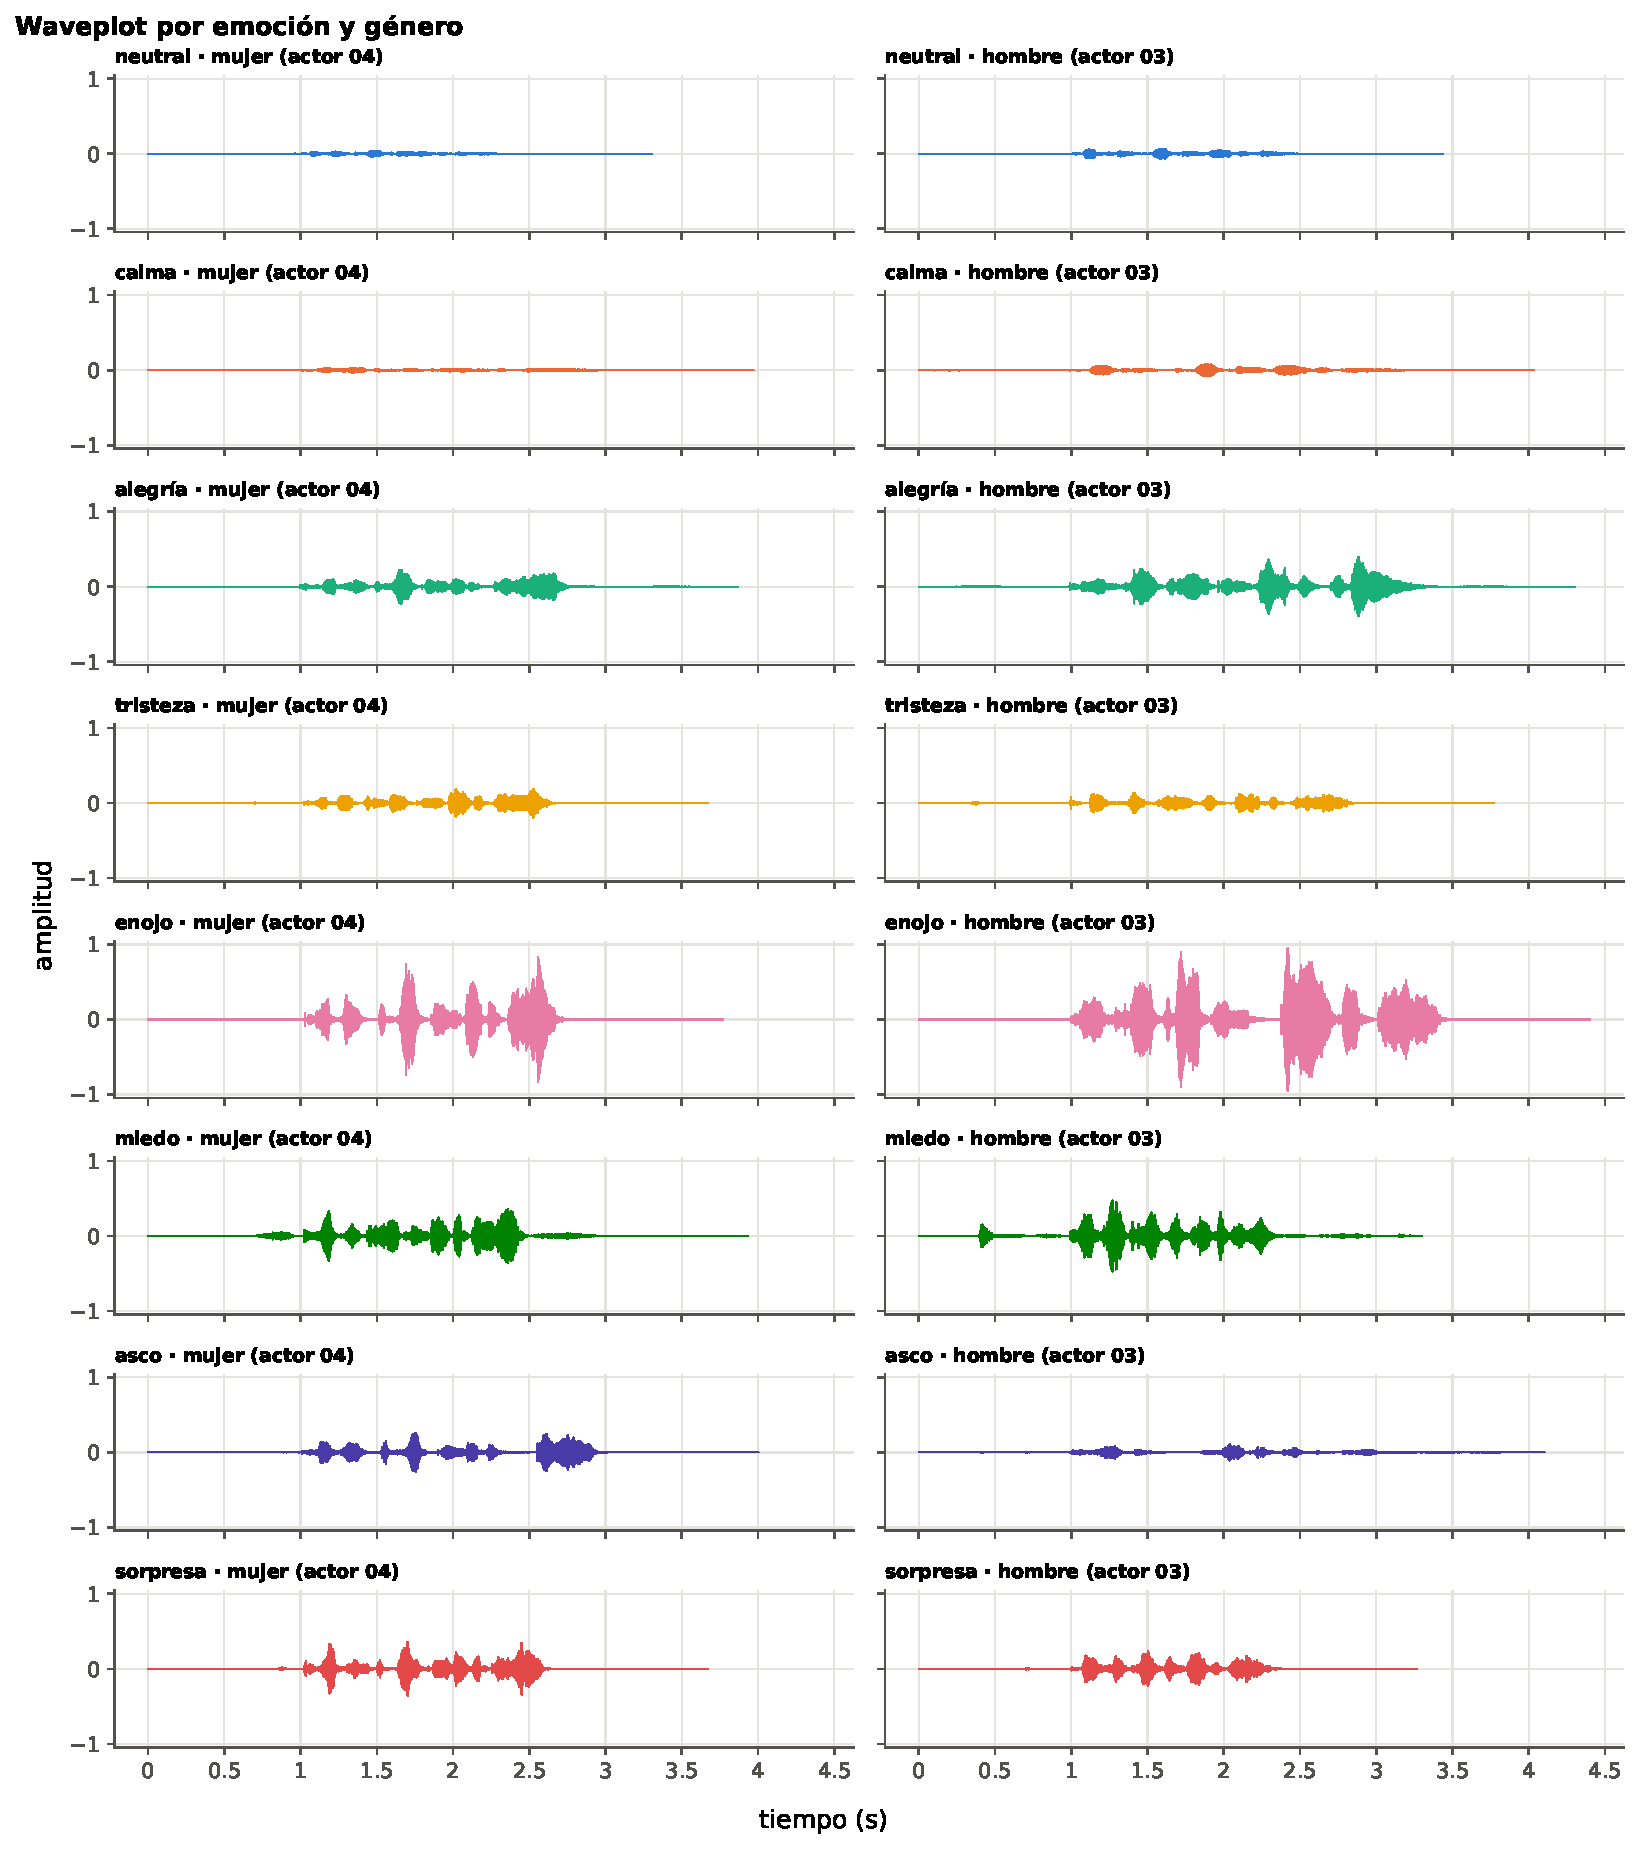
\includegraphics[height=0.82\textheight]{ondas_por_emocion}
    \end{column}
    \begin{column}{0.43\textwidth}
      \small
      \begin{itemize}
        \item Misma frase: actor 04 (mujer) y actor 03 (hombre)
        \item Enojo, alegría y miedo: mayor amplitud y ataques abruptos
        \item Neutral y calma: baja energía
        \item Asco cambia entre hablantes
      \end{itemize}
    \end{column}
  \end{columns}
\end{frame}

\begin{frame}{Envolvente de energía (todos los clips)}
  \centering
  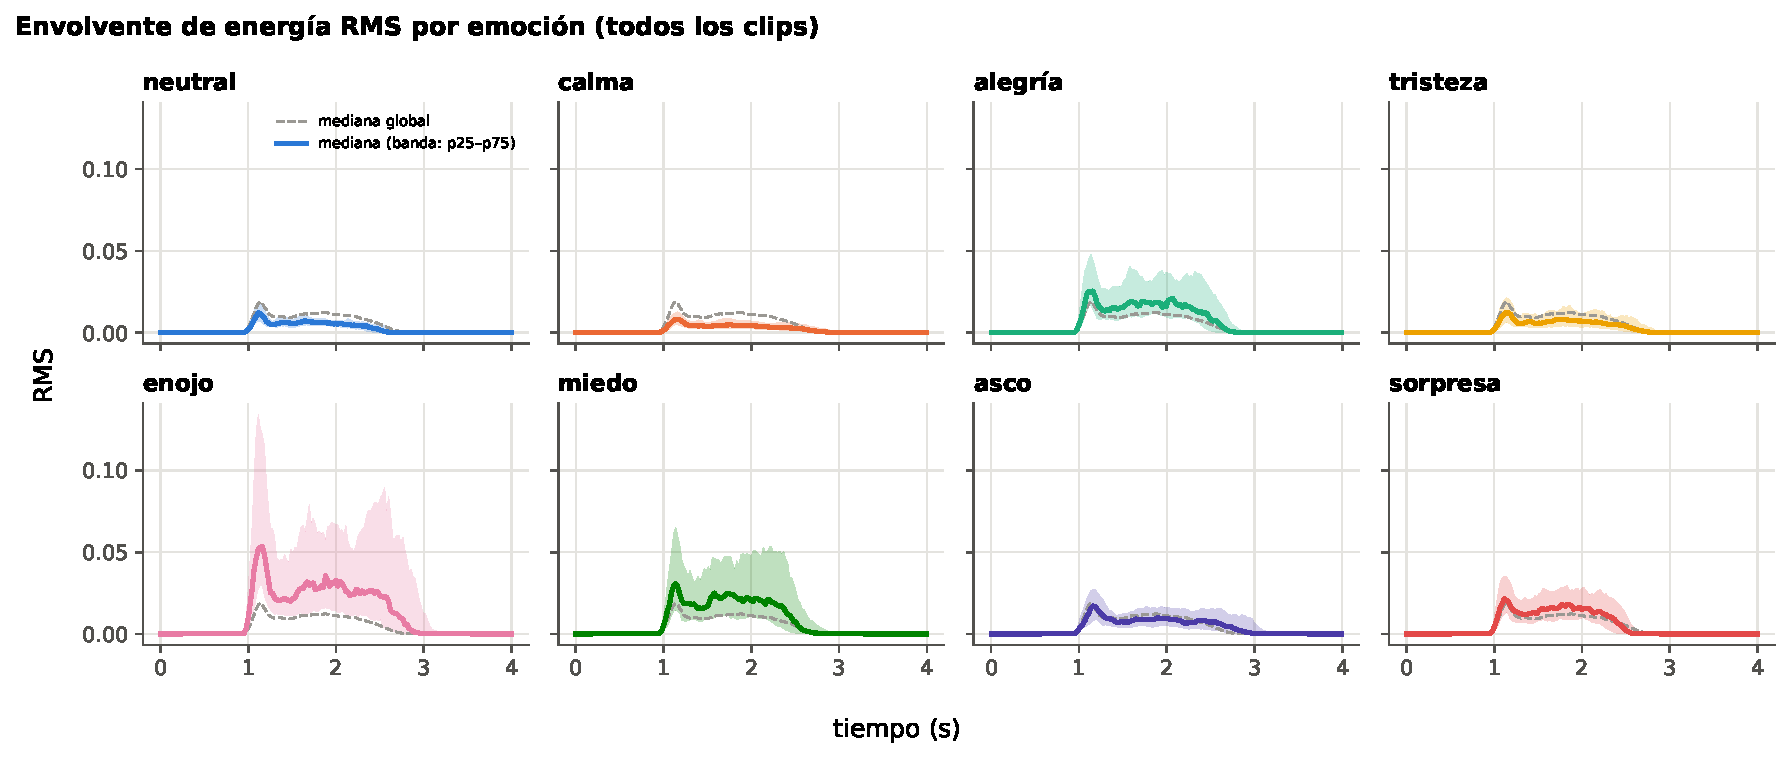
\includegraphics[width=0.84\linewidth]{envolvente_rms_por_emocion}\\[0.2em]
  \small La voz inicia en $\approx$1\,s. \textbf{Enojo} tiene el ataque y la energía más altos; asco es la
  emisión más larga.
\end{frame}

\begin{frame}{Misma frase, ocho emociones}
  \centering
  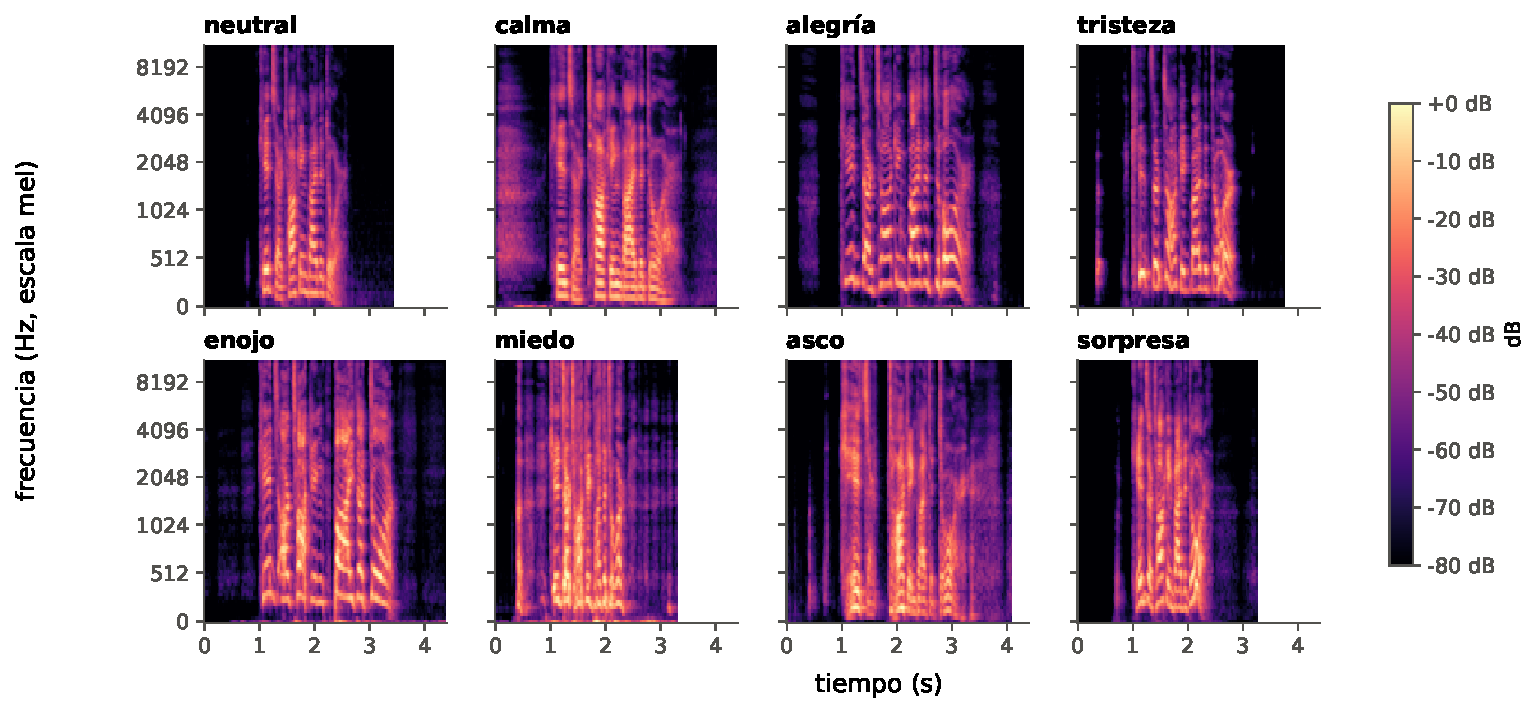
\includegraphics[width=0.78\linewidth]{espectrogramas_por_emocion}\\[0.2em]
  \small Enojo, alegría y miedo: más energía en altas frecuencias y armónicos más espaciados (tono más
  agudo).
\end{frame}

\begin{frame}{Descriptores acústicos por emoción}
  \centering
  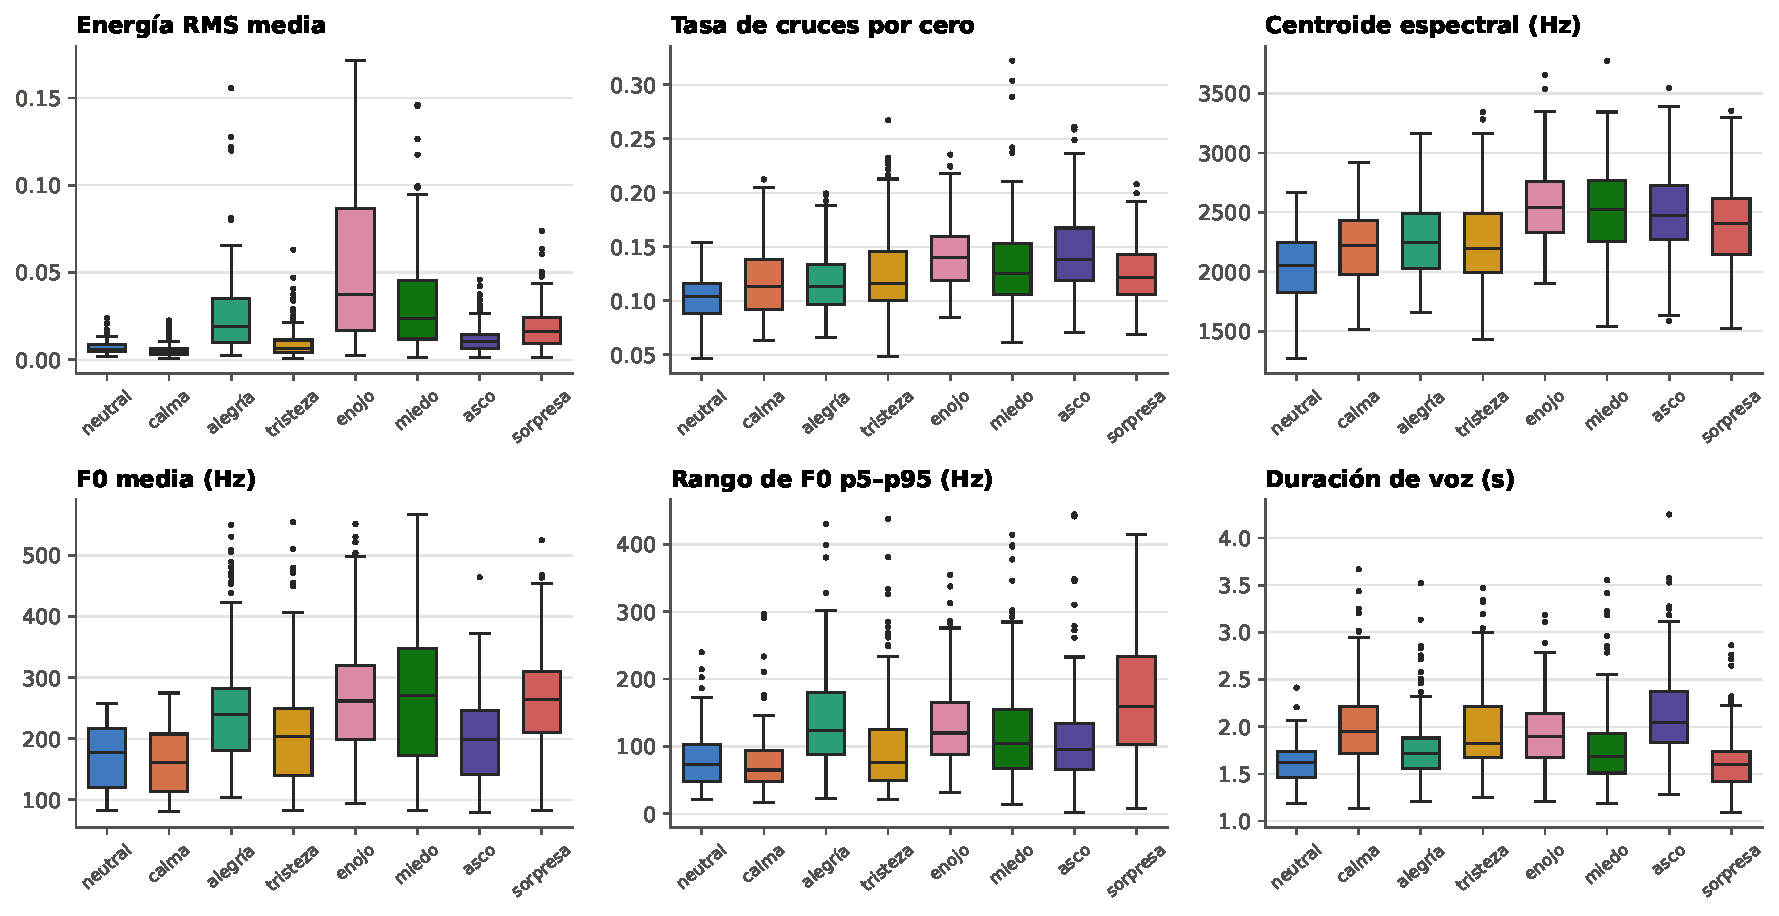
\includegraphics[width=0.84\linewidth]{descriptores_por_emocion}
\end{frame}

\begin{frame}{¿Qué descriptor distingue mejor?}
  \begin{columns}[c]
    \begin{column}{0.55\textwidth}
      \centering\small
      Kruskal--Wallis entre 8 emociones\\[0.3em]
      \footnotesize
      \begin{tabular}{@{}lrrr@{}}
        \toprule
        Descriptor & $H$ & $p$ & $\varepsilon^2$ \\
        \midrule
        \tablaKruskal
        \bottomrule
      \end{tabular}\\[0.3em]
    \end{column}
    \begin{column}{0.42\textwidth}
      \begin{itemize}
        \item \textbf{Energía}: \emoMaxRMS{} \rmsMaxVal{} vs.\ \emoMinRMS{} \rmsMinVal
        \item \textbf{F0}: \emoMaxFo{} \foMaxVal\,Hz vs.\ \emoMinFo{} \foMinVal\,Hz
        \item Ningún descriptor separa solo las 8 clases
      \end{itemize}
    \end{column}
  \end{columns}
\end{frame}

\begin{frame}{Género e intensidad}
  \centering
  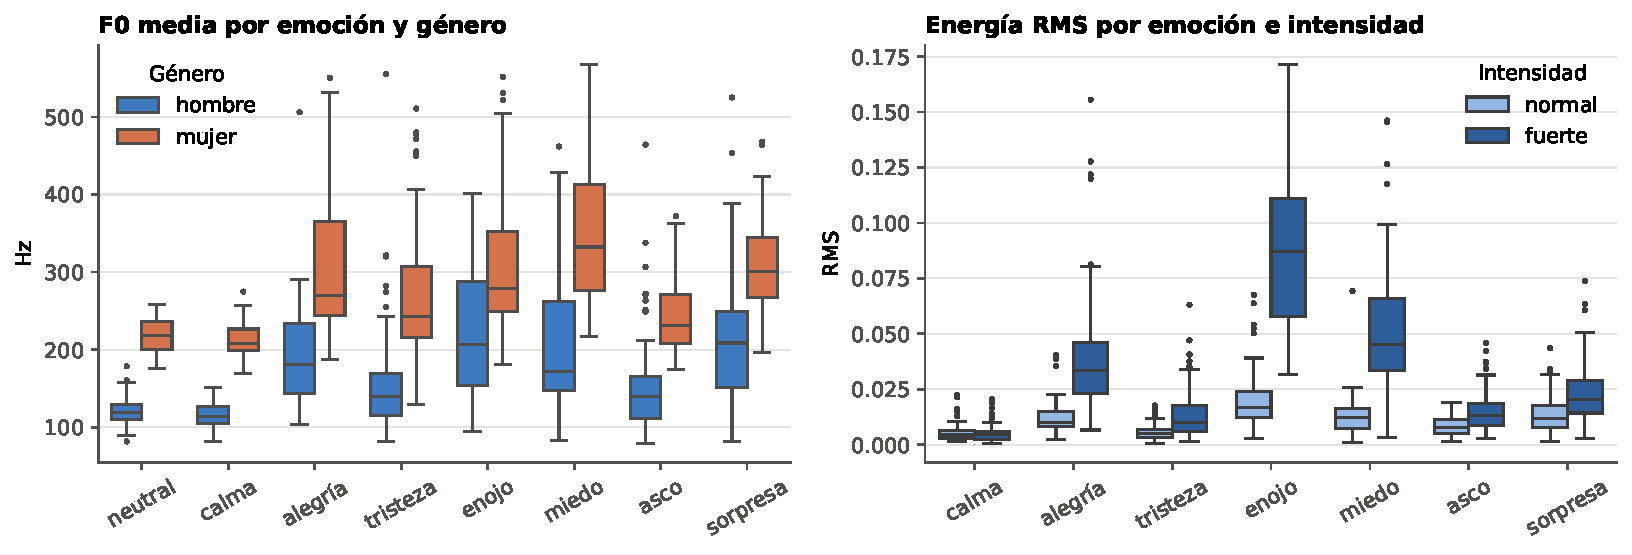
\includegraphics[width=0.9\linewidth]{genero_intensidad}\\[0.3em]
  \small F0 mediana: \textbf{\foHombre\,Hz (H) vs.\ \foMujer\,Hz (M)}, una diferencia mayor que entre
  emociones.\\
  La intensidad fuerte multiplica la energía por \textbf{\rmsRatio}.
\end{frame}

\begin{frame}{Valores atípicos por género (regla IQR)}
  \begin{columns}[c]
    \begin{column}{0.58\textwidth}
      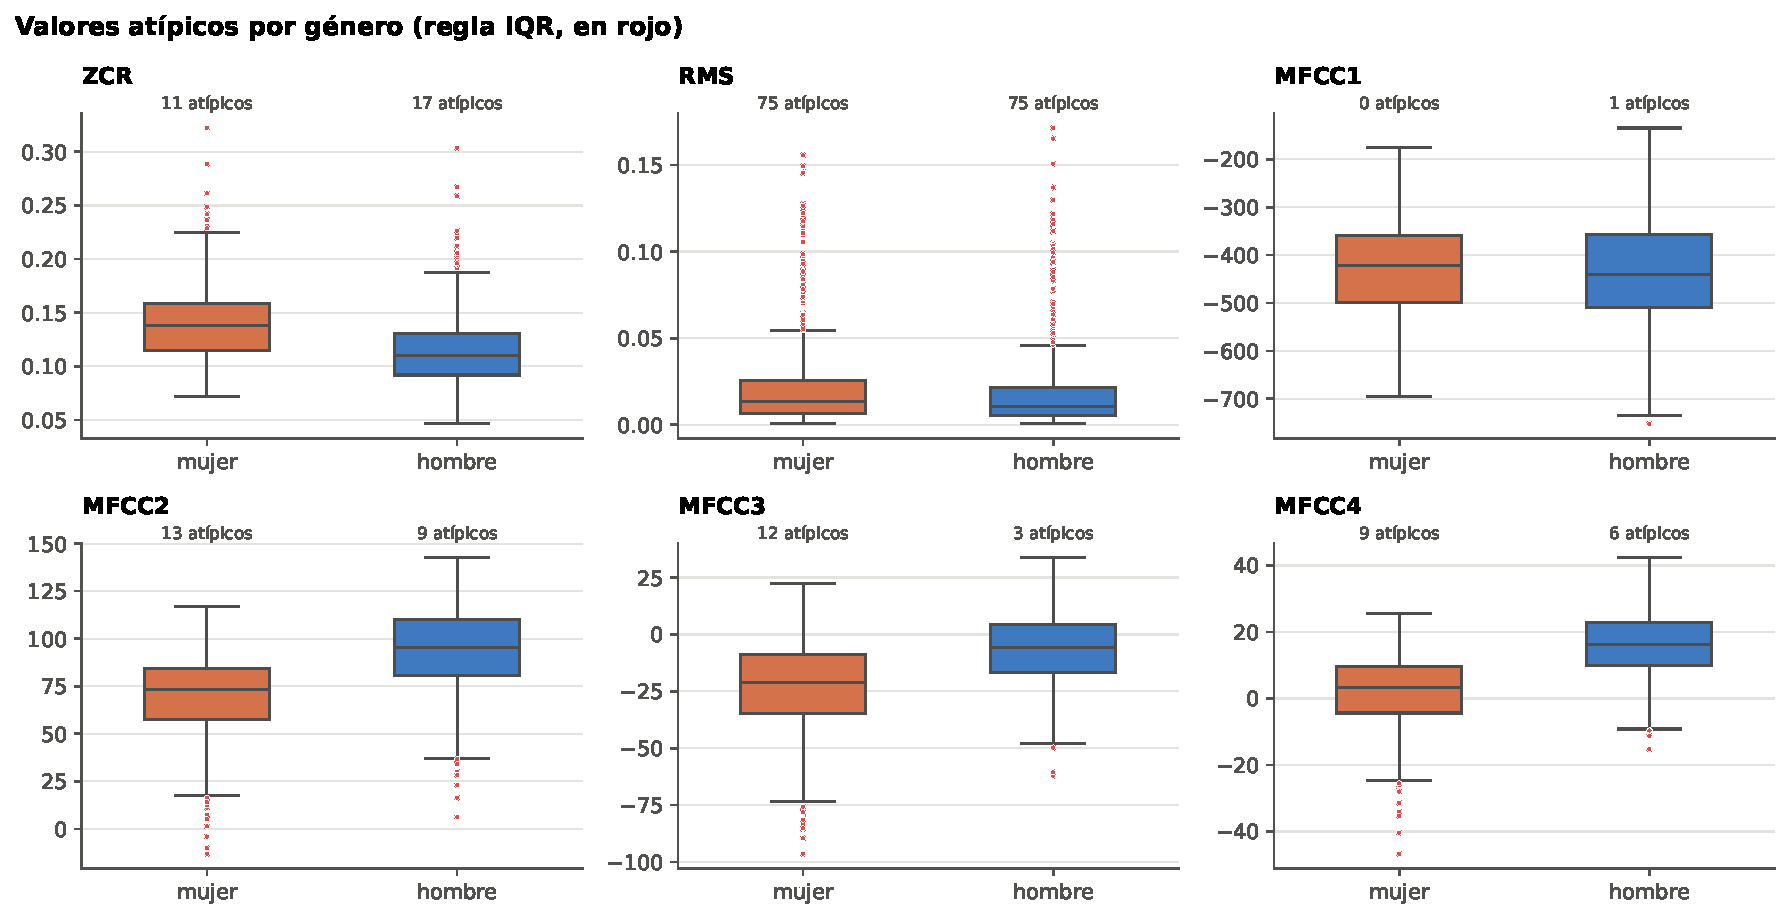
\includegraphics[width=\linewidth]{atipicos_genero}
    \end{column}
    \begin{column}{0.4\textwidth}
      \footnotesize
      \begin{tabular}{@{}lrrrr@{}}
        \toprule
        & \multicolumn{2}{c}{Mujeres} & \multicolumn{2}{c}{Hombres} \\
        & $n$ & \% & $n$ & \% \\
        \midrule
        \tablaAtipicos
        \bottomrule
      \end{tabular}\\[0.4em]
      \nota{$n=\nMujer$ clips por género.}
    \end{column}
  \end{columns}
\end{frame}

\begin{frame}{¿De dónde vienen los atípicos?}
  \centering
  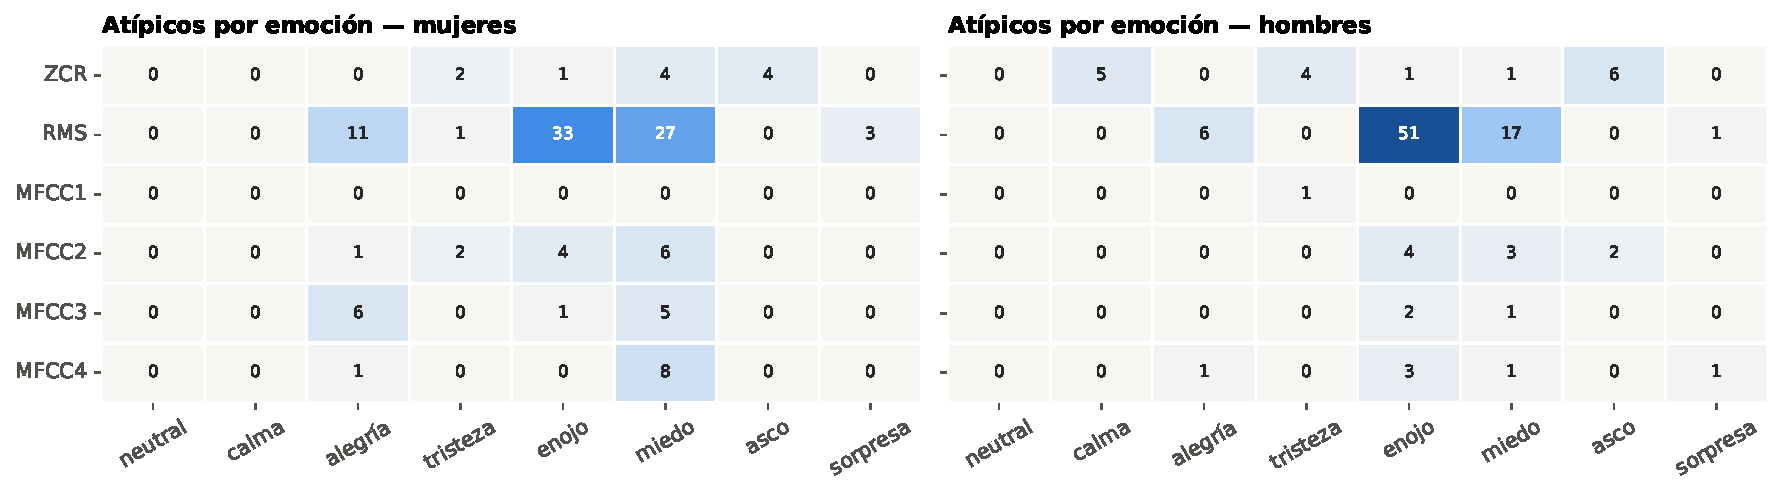
\includegraphics[width=0.95\linewidth]{atipicos_por_emocion}\\[0.4em]
  \small Los atípicos de RMS vienen de \textbf{enojo, miedo y alegría} con intensidad fuerte: son
  \textbf{señal, no ruido}.\\
  $\Rightarrow$ conservarlos y usar escalas robustas (log, cuantiles).
\end{frame}

\begin{frame}{Patrones por emoción: mujeres}
  \centering
  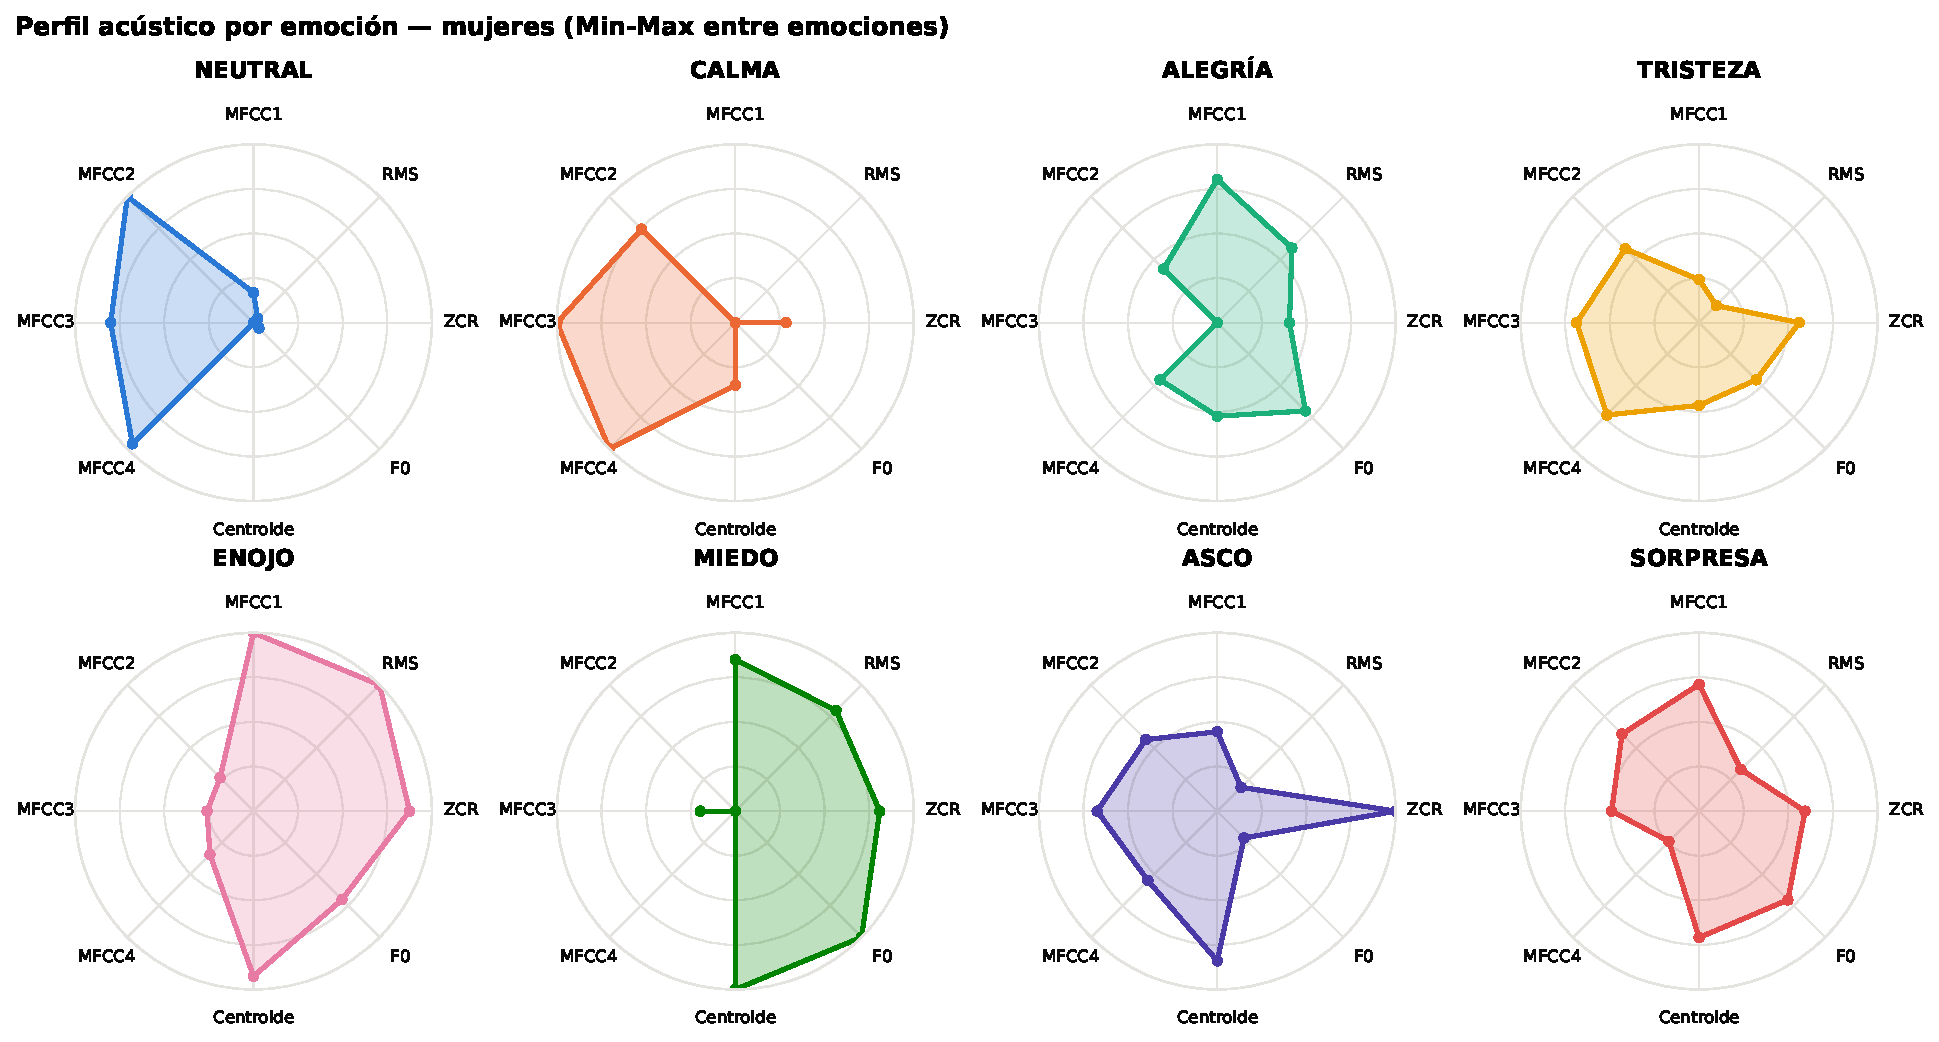
\includegraphics[height=0.8\textheight]{radar_mujeres}\\
  \nota{Media por emoción, Min-Max entre emociones dentro del género.}
\end{frame}

\begin{frame}{Patrones por emoción: hombres}
  \centering
  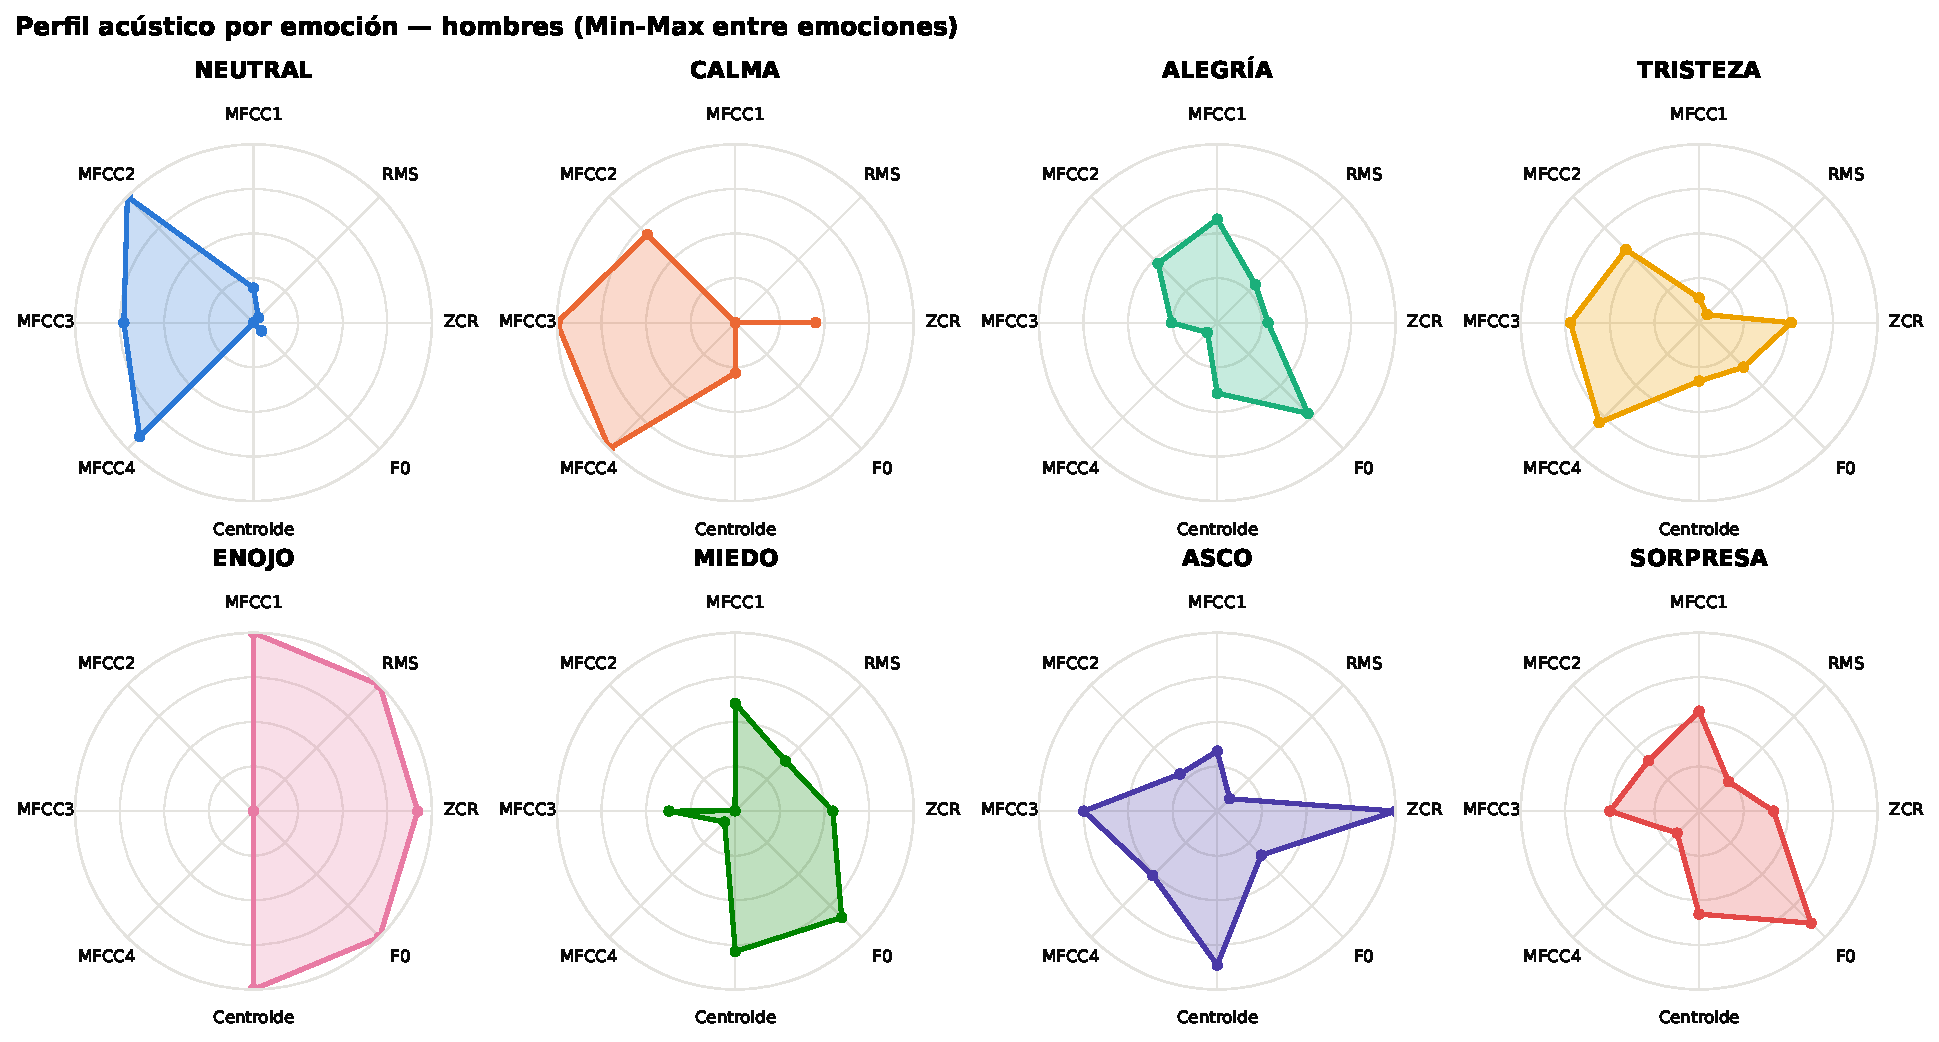
\includegraphics[height=0.8\textheight]{radar_hombres}\\
  \small Perfiles casi iguales a los de mujeres. \textbf{Enojo}: energía; \textbf{miedo/sorpresa}: tono;
  \textbf{asco}: ZCR alta con energía baja.
\end{frame}

\begin{frame}{Perfil MFCC y redundancia}
  \begin{columns}[c]
    \begin{column}{0.58\textwidth}
      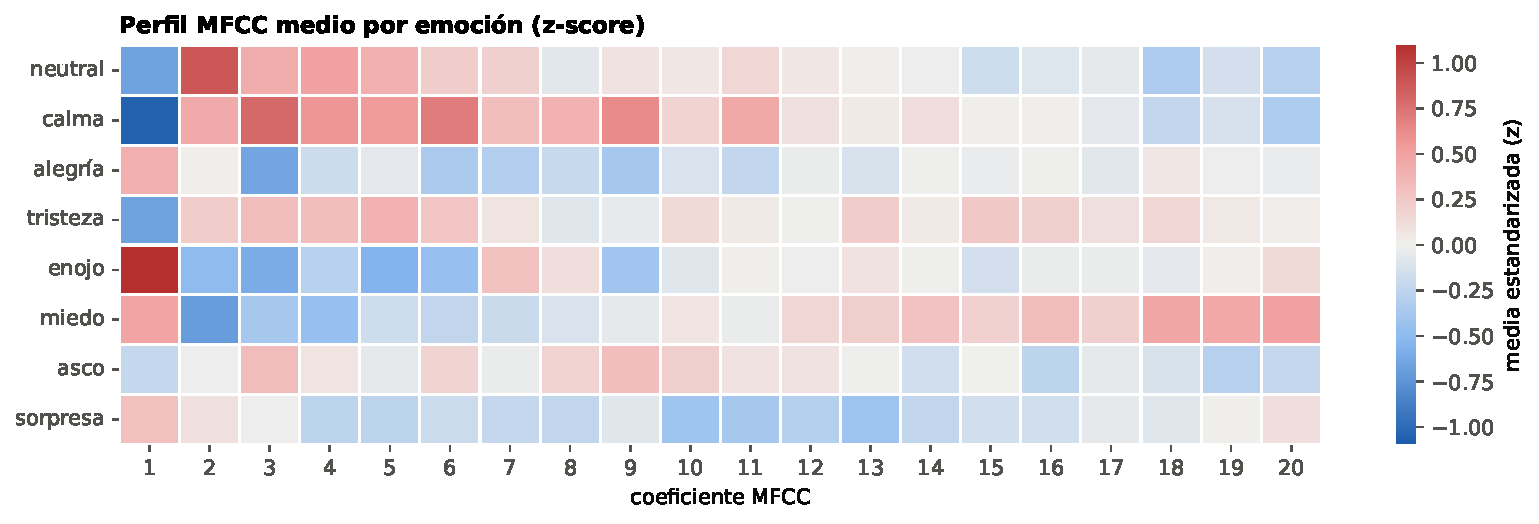
\includegraphics[width=\linewidth]{mfcc_por_emocion}\\[0.4em]
      \small MFCC1 $\approx$ energía ($\rho=0.97$). Los MFCC 2--6 separan activación baja (+) de alta (--).
    \end{column}
    \begin{column}{0.4\textwidth}
      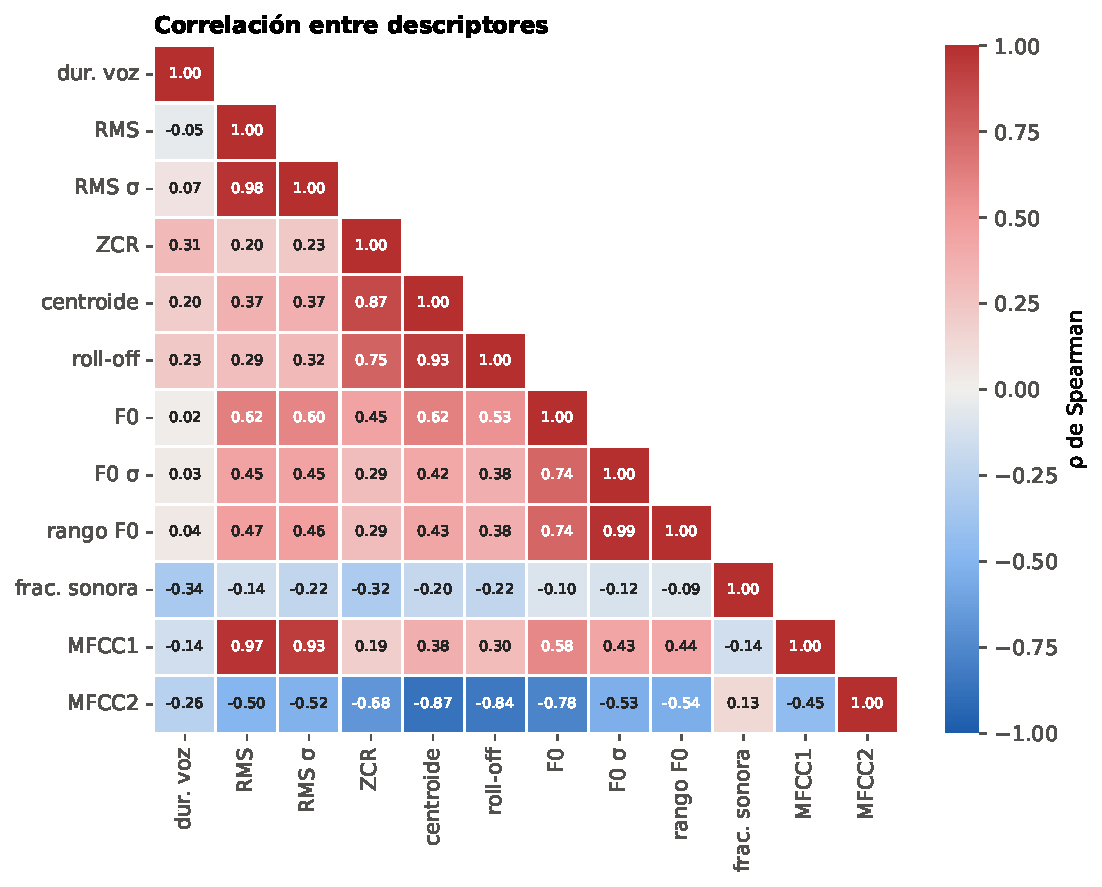
\includegraphics[width=\linewidth]{correlacion_descriptores}
    \end{column}
  \end{columns}
\end{frame}

\begin{frame}{Estructura global (PCA)}
  \centering
  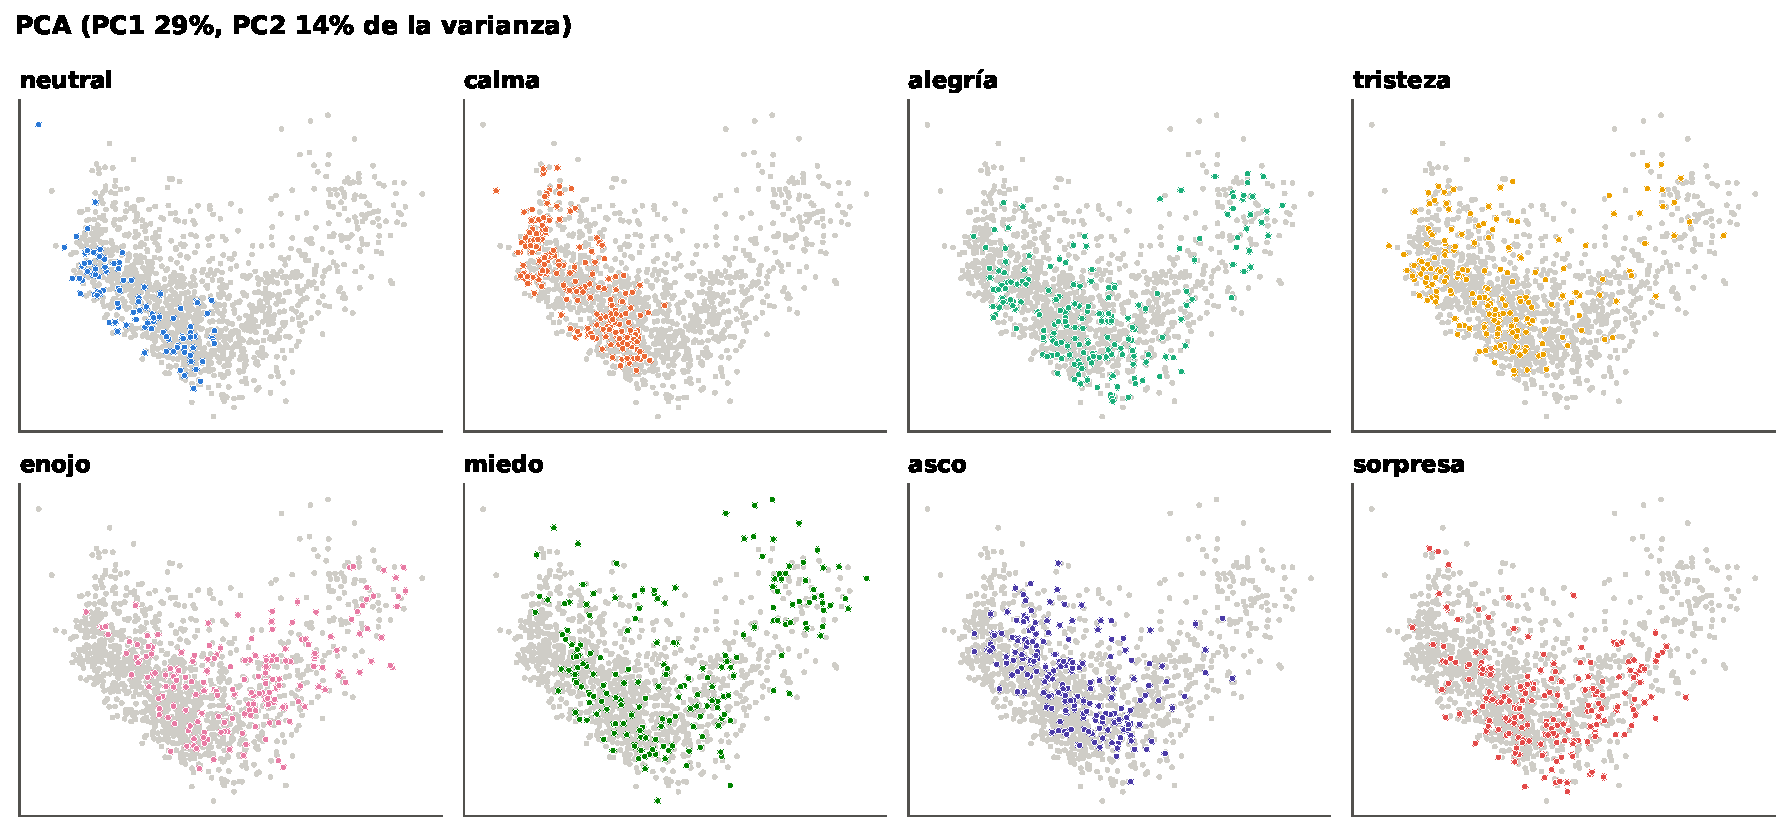
\includegraphics[width=0.84\linewidth]{pca_emociones}\\[0.2em]
  \small PC1 (\pcUno\,\%) funciona como un \textbf{eje de activación}; se necesitan \nPCNoventa{}
  componentes para el 90\,\% de la varianza.
\end{frame}

\begin{frame}{El hablante domina sobre la emoción}
  \begin{columns}[c]
    \begin{column}{0.6\textwidth}
      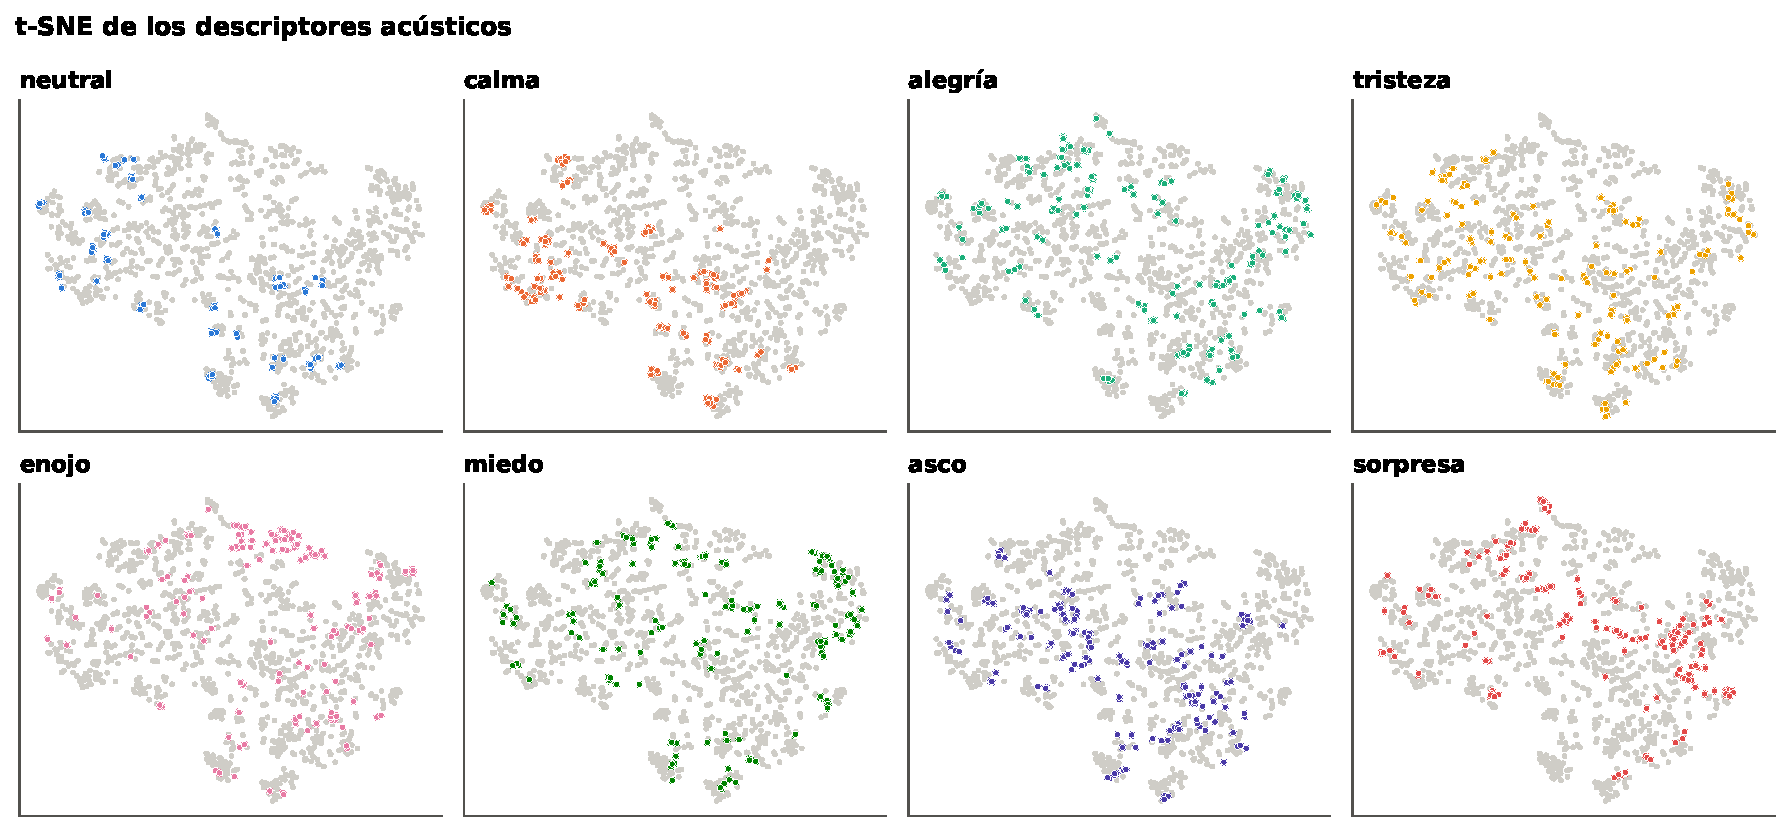
\includegraphics[width=\linewidth]{tsne_emociones}
    \end{column}
    \begin{column}{0.38\textwidth}
      \centering
      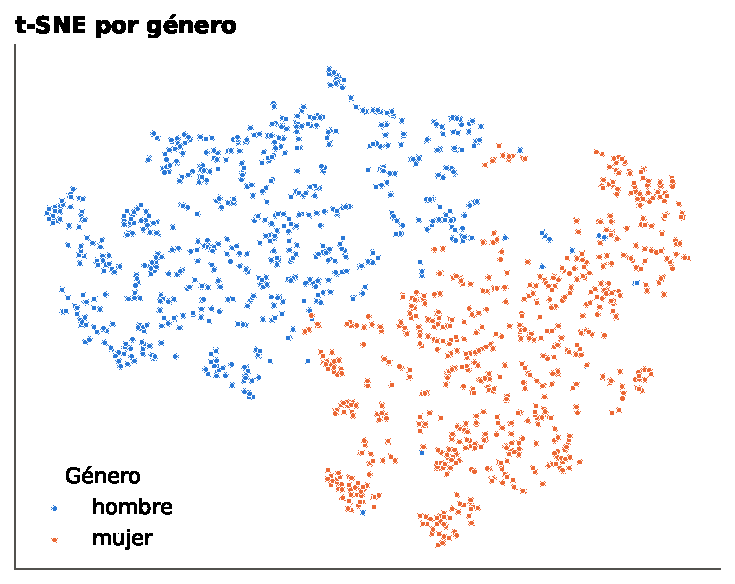
\includegraphics[width=0.85\linewidth]{tsne_genero}\\[0.3em]
      \small En t-SNE, las emociones se mezclan, mientras que el \textbf{género} forma dos regiones
      casi disjuntas.
    \end{column}
  \end{columns}
\end{frame}

% ===================== RESULTADOS =====================
\section{Resultados}
\begin{frame}{Resultados del análisis exploratorio}
  \footnotesize
  \begin{enumerate}
    \item \textbf{Datos limpios y completos}: \nClips{} clips; solo hay que convertir a mono y recortar
          silencios ($\approx$50\,\% del clip).
    \item \textbf{Balance}: perfecto por actor y género; neutral tiene la mitad de muestras.
          $\Rightarrow$ métricas macro y pesos por clase.
    \item \textbf{Señal emocional}: energía, F0, duración y centroide difieren significativamente y
          describen sobre todo un eje de \emph{activación}.
    \item \textbf{Atípicos}: concentrados en la energía ($\approx$10\,\%), propios de las emociones de alta
          activación $\Rightarrow$ conservarlos.
    \item \textbf{Radar}: perfiles por emoción compartidos entre géneros una vez normalizados.
    \item \textbf{Confusor principal}: el hablante y su género.
          $\Rightarrow$ evaluación con actores no vistos, normalización por hablante y aumentación de
          tono.
    \item \textbf{Infraestructura}: corpus en Supabase con acceso de solo lectura, reproducible desde
          cualquier equipo.
  \end{enumerate}
\end{frame}

\begin{frame}{Referencias}
  \footnotesize
  \begin{itemize}
    \item S.~R. Livingstone y F.~A. Russo (2018). The Ryerson Audio-Visual Database of Emotional Speech
          and Song (RAVDESS). \emph{PLoS ONE} 13(5): e0196391. doi:10.1371/journal.pone.0196391.
          Licencia CC BY-NC-SA 4.0.
    \item B.~McFee \emph{et al.} (2015). librosa: Audio and music signal analysis in Python.
          \emph{Proc.\ SciPy}.
    \item gemmin. Speech Emotion Recognition 90\%. Kaggle Notebook.
  \end{itemize}
\end{frame}

\end{document}
